\section{Checkning av checklistor - Robin Andersson}
\subsection{Inledning}
Vårt system ska innehålla olika typer av checklistor på olika webbsidor. Om flera användare är inne på samma sida samtidigt och en person checkar en checkruta så ska den checkrutan bli checkad för alla användare som är inne på den webbsidan.\\

Checklistan kommer att implementeras med hjälp av html, javascript och jquery samt Socket.IO.

\subsubsection{Syfte}
Syftet med denna del av projektet är att flera sjuksköterskor samtidigt ska kunna förbereda operationer genom att plocka olika artiklar samt förbereda operationssalen och checka av det som är utfört utan att det ska bli några konflikter med att flera sjuksköterskor plockar samma artikel eller liknande.

\subsubsection{Frågeställning}
\begin{itemize}
\item Går det att anpassa checklistan för en surfplatta medan den samtidigt innehåller information om var artiklar befinner sig samt hur många av varje artikel som behövs?
\item Kommer Socket.IO vara tillräckligt snabbt för att flera personer ska kunna checka av artiklar samtidigt utan förvirring?
\end{itemize}

\subsubsection{Avgränsningar}
Eftersom denna del av projektet endast innehåller checkande av checklistor så saknas etiska aspekter.

\subsection{Teori}
Huvuddelen i implementeringen av checklistan är kommunikationen med Socket.IO som är en modul till Node.JS. Socket.IO använder sig av websockets för att kommunicera mellan front-end och back-end. Med hjälp av socket.IO så kan man skicka data från en klient till alla andra anslutna klienter och visa datan som skickades utan att någon sida behöver laddas om.
Socket.IO har olika komponenter för front-end och back-end. Händelser som skickas från den ena sidan hanteras av motsvarande händelsehanterare på den andra sidan. Varje händelse identifieras med hjälp av en sträng. Det finns några färdiga händelser i socket.io exempelvis händelsen "connection" på serversidan fås då en klient har anslutit till socket.io. \cite{socketBook} \\

För mer information om Socket.IO se deras officiella hemsida: \url{http://socket.io/}\\

HTML står för Hypertext Markup Language och är ett sidbeskrivnings språk. \cite{html} Jag kommer att behöva HTML till att ge en grafisk representation av checklistan till användarna.\\

 
\subsection{Metod}
Jag började med att fundera på hur kommunikationen skulle fungera på för sätt. Jag skissade ner olika förslag på ett papper och kom på det sättet fram till hur jag skulle implementera kommunikationen. Sedan implementerade jag den och fick den att fungera. Därefter så refaktoriserade jag koden för att få den kortare och mer lättläst.

\subsection{Resultat}
Jag kom fram till att när en användare går in på en operationsförberedelse så kommer denne in i ett rum. Varje gång en person sedan checkar en checkbox så skickas ett Socket.IO meddelande till servern som innehåller information om vilken checkruta som ska checkas samt vilket rum checkboxen ska checkas i. Servern skickar sedan ett meddelande till det givna rummet vilken checkruta som ska checkas och alla klienter som är anslutna till det rummet checkar den givna checkrutan. \\

Figuren nedan visar detta flöde i ett sekvens liknande box-and-line-diagram.
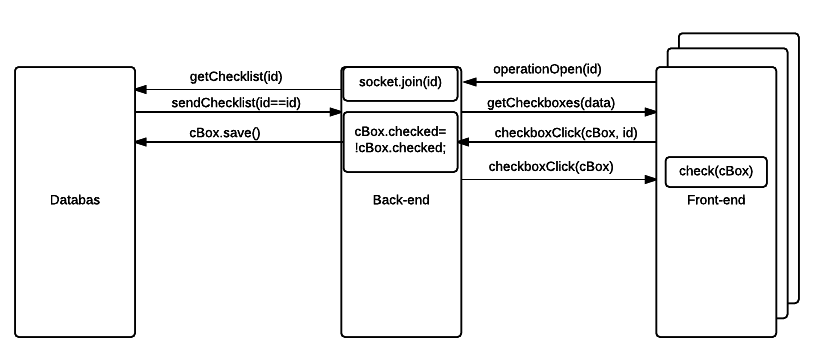
\includegraphics[scale=0.5]{checklistdiagram}\\

När två klienter går in på en operation och en klient checkar en checkruta för första gången tar det strax under en sekund innan checkrutan checkas för den andra klienten. Därefter när någon klient checkar en checkruta så kan jag inte se någon fördröjning alls från det att en klient checkar en checkruta och en annan klient får den checkrutan checkad.\\

Kunden har prövat att ha flera personer inne på samma plocklista samtidigt och checka av olika artiklar. Kunden tyckte att det fungerade bra och påpekade inte någon fördröjning. \\

All information som krävs för plocklistorna fick plats utan att det blev för plottrigt.

\subsection{Diskussion}
\subsubsection{Resultat}
Eftersom jag endast skickar data om vilken checkruta som ska checkas till de klienter som är inne på den operation som checkrutan blev checkad på så uppdateras checkningar snabbare än att göra den enkla lösningen att bara skicka datat till alla anslutna klienter. Att det tar nästan en sekund för en checkning att uppdateras på andra klienter för första gången är långsammare än förväntat. Men eftersom det endast gäller just första artikeln och att kunden har testat checkning med flera personer samtidig utan att märka några problem så verkar detta inte vara något praktiskt problem. Att en checkning sedan kan uppdateras nästan helt utan fördrdröjning var bättre än vad jag hade förväntat mig.

\subsubsection{Metod}
Den metod jag använde mig av fungerade bra, men jag tror att jag skulle kunnat komma fram till samma resultat snabbare genom att göra kortare funktioner och vettigare namn redan från början istället för att göra något som funkar så snabbt som möjligt och sedan refaktorisera. För nu blev det väldigt förvirrande kod från början och jag var tvungen att sitta och tänka på vad kod jag skrivit faktiskt gjorde. Men att skissa olika förslag på ett papper först tror jag var en väldigt bra idé, det gjorde att jag fick några möjliga lösningar och sedan kunde jag överväga fördelar och nackdelar med de olika lösningarna för att sedan välja den som verkade bäst.

\subsection{Slutsatser}
Eftersom det fungerar bra med checkning av checklistor med hjälp av socket.io och all nödvändig information får plats utan att det upplevs som plottrigt så uppfylls syftet med denna del av projektet och min frågeställning har blivit besvarad.

\subsection{Referenser}
\vspace{-9mm}
\begin{thebibliography}{9}
\bibitem{socketBook} Rai, Rohit. Socket. IO Real-Time Web Application Development. Birmingham: Packt Publishing Ltd., 2013.
\bibitem{html}\url{http://tools.ietf.org/html/draft-ietf-iiir-html-00}
\end{thebibliography}